\documentclass[11pt,hidelinks]{article}

\newcommand{\projecttitle}{BIOS 731: Final Report}
% \newcommnad{\projectsubtitle}{The Health Discovery and Well Being study: An analysis of the association between age and pulse wave velocity, and a predicted regression model for pulse wave velocity}
\newcommand{\duedate}{Spring 2026}
\newcommand{\authorname}{Randy Parrish}

% Load packages
\usepackage[T1]{fontenc}
% \usepackage{fontspec}
% \setmainfont{Arial}
\usepackage[utf8]{inputenc}
% \usepackage{uarial}
\usepackage[toc,page]{appendix}


\let\oldthebibliography\thebibliography
\renewcommand{\thebibliography}[1]{%
  \oldthebibliography{#1}
  \let\oldbibitem\bibitem
  \let\oldtextsc\textsc
  \def\oldbbland{et}
  \newcounter{authorcount}
  \def\bibitem[##1]##2{%
    \let\textsc\oldtextsc
    \let\bbland\oldbbland
    \oldbibitem[##1]{##2}%
    \let\textsc\mytextsc%
    \let\bbland\mybbland
    \setcounter{authorcount}{0}
  }
  \def\mybbland{\setcounter{authorcount}{0}\oldbbland}
  \def\dropetal##1.{ \bbletal}
  \def\mytextsc##1{%
    \oldtextsc{##1}%
    \stepcounter{authorcount}%
    \ifnum\value{authorcount}=5\relax%
      \expandafter\dropetal%
    \fi%
  }%
}




\usepackage[fleqn]{amsmath} %left flush equations
\usepackage[margin=0.75in,top=0.75in,bottom=0.75in]{geometry} %set margins
\usepackage{amssymb} %additional math symbols
\usepackage{bm} %bold math symbols
\usepackage{booktabs} %tables
\usepackage{caption} %captions for tables
\usepackage{fancyhdr} %formatting header
\usepackage{float} %better float positioning
\usepackage{hyperref} %clickable links
\usepackage{indentfirst}
\usepackage{longtable}
\usepackage{graphicx}
\usepackage[square, sort, numbers]{natbib} %bibliography stuff
\usepackage{setspace} %spacing section headers
\usepackage{subcaption}
\usepackage{titlesec} %formatting section headers
\usepackage{listings} %formatting code blocks
\usepackage{xcolor}
\xdefinecolor{gray}{rgb}{0.5,0.5,0.5}
\xdefinecolor{blue}{rgb}{0.0,0.0,1.0}
\xdefinecolor{darkblue}{rgb}{0.0,0.2,0.6}
\xdefinecolor{green}{rgb}{0.0,0.5,0.0}
\lstset{language=R, 
  breaklines=true,  
  basicstyle=\small\ttfamily\color{black},
  columns=fixed,
  keepspaces=true,
  keywordstyle=\color{darkblue},
  stringstyle=\color{purple},
  commentstyle=\rmfamily\itshape\color{gray},
  numberstyle=\color{green},
  alsoletter={.<-},% becomes a letter
  alsoother={$},% becomes other
  otherkeywords={data.frame,is.na,rowSums,rowMeans,$},
  morekeywords={in,c},
  deletekeywords={C}% remove keywords
  }
\usepackage{pdflscape}
\usepackage{afterpage}
  
% formatting
\let\proglang=\textsf
\let\code=\texttt

%Section header spacing
% \titlespacing{\section}{1pt}{1em}{1em}
\titlespacing{\subsection}{0em}{1em}{0.5em}
\titlespacing{\subsubsection}{\parindent}{0.75em}{0.5em}

% %Section header formatting
% \titleformat{\section}{\bfseries\scshape}{\thesection}{0.75em}{}[]
% \titleformat{\subsection}{\bfseries}{\thesubsection}{0.75em}{}[]
% \titleformat{\subsubsection}[runin]{\itshape}{}{0.5em}{}[.\ ]

%Title stuff
\title{\projecttitle}
\author{Randy Parrish}
\date{\duedate}

%Header
\pagestyle{fancy}
\lhead{Randy Parrish}
\chead{\projecttitle}
\rhead{\duedate}

% \usepackage{titling}
% \setlength{\droptitle}{-2cm}


\newenvironment{tightcenter}{%
  \setlength\topsep{2pt}
  \setlength\parskip{2pt}
  \begin{center}
}{%
  \end{center}
}

\usepackage{cleveref}

%Start of document
\begin{document} 

% % increase \bibhang to take care of the numbers
% \setlength{\bibhang}{2pc}
% \makeatletter
% % patch \@lbibitem to print the current number before the authors
% \patchcmd{\@lbibitem}
%   {]}
%   {][\theNAT@ctr] }
%   {}{}
% \makeatother

\clearpage%\maketitle
\thispagestyle{empty}

\begin{tightcenter}
{\centering\Large\textbf{\projecttitle}}\\
{\centering\large\authorname}\\
{\centering\duedate}
\end{tightcenter}

% ABSTRACT
\begin{abstract}
\noindent\normalsize 
Traditional transcriptome-wide and proteome-wide association studies (TWAS/PWAS) limit analyses to \textit{cis}- molecular quantitative trait loci (xQTL), neglecting \textit{trans}-xQTL that compose a substantial proportion of molecular variation. The BGW-xWAS tool implements a Bayesian-Genome Wide (BGW) framework based upon a Bayesian variable selection regression (BVSR) model that jointly accounts for both \textit{cis}- and \textit{trans}-xQTL factors to improve genetically-regulated gene expression (GReX) and protein abundance (GReP) imputation accuracy and xWAS power over \textit{cis}-only methods. To study both \textit{cis}- and \textit{trans}- regulatory mechanisms of AD, this study applies the BGW-xWAS tool to train xWAS models of dorsolateral prefrontal cortex tissue from ROS/MAP and integrates the results with large genome-wide association study (GWAS) summary data of Alzheimer disease (AD) dementia in order to identify genetically-regulated molecular associations underlying AD risk.


\end{abstract}
% \newpage
%%%%%


\section{Introduction}
Traditional xWAS analyses neglect the importance of distant xQTL factors (i.e., \textit{trans}-eQTLs located outside of the $\pm$1 MB region) that possess a key role in molecular variation. In highly polygenic neurodegenerative disease (e.g., Alzheimer's disease (AD)), genome-wide TWAS analyses that jointly model \textit{cis}- and \textit{trans}-eQTLs have shown that roughly one-quarter to one-third of significant AD risk genes across brain and blood are predominantly driven by \textit{trans}-eQTL weights. This includes 34 of 141 genome-wide significant genes in a recent Bayesian TWAS of AD dementia, indicating that \textit{cis}-only models miss a substantial fraction of disease-relevant regulatory effects~\cite{guoBayesianGenomewideTWAS2024}. 

The BGW-TWAS tool~\cite{luninghamBayesianGenomewideTWAS2020} was developed in order to circumvent the computational burden of incorporating \textit{trans}- variants into TWAS analyses. In this paper the underlying models used by the BGW-xWAS tool are described. An application TWAS and PWAS of AD is conducted to study the impacts of the \textit{cis}- and \textit{trans}- regulatory mechanisms of AD dementia using the BGW-xWAS tool to account for \textit{cis}- and \textit{trans}-xQTL factors to improve genetically regulated gene expression (GReX) imputation accuracy and xWAS power over \textit{cis}-only methods~\cite{luninghamBayesianGenomewideTWAS2020}. 


\subsection{Standard Two-Stage xWAS} %
The standard two-stage xWAS methods~\cite{gamazonGenebasedAssociationMethod2015, gusevIntegrativeApproachesLargescale2016, nagpalTIGARImprovedBayesian2019,huProteomewideAssociationStudies2025} first fit gene quantitative trait (genetically-regulate gene expression (GReX), genetically-regulated protein abundance (GReP)) prediction models using the reference -omic and genetic data profiled for the same samples, and then test the association between the predicted genetically regulated quantitative trait (GReX or GReP) and phenotype of interest for the test GWAS cohort. Given a reference genotype, $\textbf{G}_0$, and quantitative trait (gene expression, protein abundance, etc.), $\textbf{Q}_0$, data from the same subjects, 
\[\textbf{Q}_0 = \textbf{G}_0 \textbf{w} + \boldsymbol{\epsilon}, \qquad \boldsymbol{\epsilon} \sim N(0,\, \sigma^2_{\epsilon}\textbf{I})\]
where $\textbf{w}$ is xQTL weights. In step 2, the association between predicted genetically-regulated quantitative trait (GReX or GReP) and phenotype of interest xQTL weights $\hat{\textbf{w}}$ estimated in step 1: 
\[\widehat{\textbf{GReX}} = \textbf{G}_{\text{test}} \hat{\textbf{w}}\]



\section{BGW-xWAS Tool}

Although \textit{trans}-SNPs explain much variation in expression quantitative traits, and may be significant themselves, existing TWAS tools only considered \textit{cis}-SNPs (variants within $\pm$1MB of a gene). Including \textit{trans}- variants expected to increase imputation accuracy of GReX and the power of TWASs, however, routine TWAS methods are impractical given the computational cost required to fit 20K GReX imputation models for genomewide genes and 10M genotypes per tissue. The BGW-TWAS tool~\cite{luninghamBayesianGenomewideTWAS2020} was developed in order to circumvent this computational burden. While it was originally developed for TWAS, the same software can be applied to other kinds of QTLs; in this context, the tool is referred to as "BGW-xWAS".

In order to reduce computational burden, BGW-xWAS employs a scalable EM-MCMC algorithm and uses summary statistics of standard eQTL analyses based on single variant tests. Dependencies include C++ libraries zlib, gsl, eigen3, lapack, atlas, blas, and libStatGen\cite{StatgenLibStatGen2024}. For computational efficiency, it is recommended these libraries and scripts for the tool itself be compiled by the user.

\subsection{Bayesian variable selection regression (BVSR)}
The eQTL effect size $w_i$ follows a "spike-and-slab" prior distribution–ie, we only retain a subset of the possible regressors; $w_i$ follows a $ N(0, \sigma_w^2\sigma_{\epsilon}^2)$ distribution with probability $\pi$ and $w_i$ follows point-mass density function $\partial_0(\cdot)$ (ie, is 0) with probability $1-\pi$. If $w_i=0$ then $\partial_0(w_i)=1$, otherwise $\partial_0(w_i)=0$. 
\[\textbf{E}_{g, n\times 1} = \textbf{X}_{n\times p} \textbf{w}_{p\times1} + \boldsymbol{\epsilon}_{n\times 1},\qquad w_i\sim \pi N(0, \sigma_w^2\sigma_{\epsilon}^2) + (1-\pi)\partial_0(\cdot),\qquad \epsilon_i\sim N(0,\sigma_{\epsilon}^2)\]

The BVSR model is expanded to include both \textit{cis}- and \textit{trans}- variants:
    \begin{align*}
      \textbf{E}_g &= \textbf{X}_{\textnormal{cis}}\textbf{w}_{\textnormal{cis}} +  \textbf{X}_{\textnormal{trans}}\textbf{w}_{\textnormal{trans}} + \boldsymbol{\epsilon}, \qquad\qquad  \epsilon_i\sim N(0,\sigma_{\epsilon}^2) \\
      w_{\textnormal{cis},i} &\sim \pi_{\textnormal{cis}}N(0, \sigma^2_{\textnormal{cis}}\sigma_{\epsilon}^2) + (1-\pi_{\textnormal{cis}}) \partial_0(w_{\textnormal{cis},i}), \qquad 
      w_{\textnormal{trans},i} \sim \pi_{\textnormal{trans}}N(0, \sigma^2_{\textnormal{trans}}\sigma_{\epsilon}^2) + (1-\pi_{\textnormal{trans}}) \partial_0(w_{\textnormal{trans},i})
    \end{align*}

The model assumes independent conjugate hyper priors:
    \begin{align*}
    	\pi_{\textnormal{cis}} &\sim Beta(a_{\textnormal{cis}}, b_{\textnormal{cis}}), \;\qquad\qquad \sigma^2_{\textnormal{cis}} \sim IG(k_1,k_2) \qquad\qquad \sigma^2_{\epsilon}\sim IG(k_3,k_4) \\
    	\pi_{\textnormal{trans}} &\sim Beta(a_{\textnormal{trans}}, b_{\textnormal{trans}}),\qquad \sigma^2_{\textnormal{trans}} \sim IG(k_3,k_4)
    \end{align*}


To further reduce computational burden, a latent indicator vector $\boldsymbol{\gamma}_{p\times 1}$ is introduced to aide computation. Each element $\gamma_i$ indicates whether $w_{\cdot,i}=0$ ($\gamma_i=0$) or follows the $N(0,\sigma_{\cdot}^2\sigma_{\epsilon}^2)$ distribution ($\gamma_i=1$). $\textnormal{E}(\gamma_i)$ is the posterior probability ($\textnormal{PP}_i$) for the $i$th SNP to be an eQTL with non-zero effect size $w_i$.

\subsection{Efficient Computation Using EM-MCMC}
While eQTL effect sizes and posterior probabilities $(\hat{w}_i, \widehat{PP}_i)$ could be obtained with a standard Markov Chain Monte Carlo (MCMC) algorithm, this is not feasible for genome-wide modeling due to slow convergence rate and large memory usage. Instead, BGW-TWAS further adapts an existing scalable expectation maximization EM-MCMC to use only summary statistics, incliding linkage disequillibrium and score statistics from standard eQTL analyses by single variant tests. Genotype regions are further pruned to reduce computational burden. 

During the E-step, the EM-MCMC algorithm uses MCMC per genome block (in parallel) to estimate $(\textbf{w},\textbf{PP})$ from most recent estimation of $(\boldsymbol{\pi},\boldsymbol{\sigma}^2)$. During the M-step, the newly obtained $(\boldsymbol{\pi},\boldsymbol{\sigma}^2)$ is used to update $(\boldsymbol{\pi},\boldsymbol{\sigma}^2)$. Iterations continue until maximum a posteriori (MAP) estimates converge. Once the final estimates $( \hat{\textbf{w}}, \widehat{\textbf{PP}} )$ are obtained, estimated GReX is calculated:
\[\widehat{\textbf{GReX}} = \sum_{i=1}^p \tilde{X}_i(\widehat{PP}_i\hat{w}_i) \]


\subsection{Summary-Level Association Test}
A burden Z-score as implemented by S-PrediXcan\cite{barbeiraExploringPhenotypicConsequences2018} can be used to test the association between predicted GReX and a phenotype of interest. 

\[{\widetilde{Z}_g} = \sum_{i \in \text{Model}} \frac{ (\widehat{PP_{i}}\,\widehat{w_{i}}) \; \widehat{\sigma_{i}}\; Z_{\textnormal{GWAS},i} }{ \sqrt{(\widehat{\vec{PP}}\,\widehat{\vec{w}})'\;\vec{V}\;(\widehat{\vec{PP}}\,\widehat{\vec{w}})} },\qquad\widehat{\sigma_{i}^{2}} = \text{Var}(\vec{G}_{0,i}),\qquad\vec{V} = \text{Cov}(\vec{G}_{0})\]

where  $\widehat{PP_{i}}$ is the estimated posterior causal probability for SNP $i$, $\widehat{w_{i}}$ is theestimated xQTL effect-size for SNP $i$,$Z_{\textnormal{GWAS},i}$ is the Z-score statistic values for single variant test (ie, GWAS), $\widehat{\vec{PP}}$ is the estimated posterior causal probabilities from trained model,${\widehat{\vec{w}}}$ is the xQTL effect-sizes from trained model, $\vec{V}$ is the genotype covariance matrix (LD data) estimated from reference panel genotype data $\vec{G}_0$, $\vec{G}_{0}$ is the reference genotype matrix, and $\widehat{\sigma_{i}}$ is the estimated standard deviation of SNP $i$ from genotype vector for SNP $i$, $\vec{G}_{0,i}$.


\section{Methods} 

\subsection{ROS/MAP Dataset} %
The Religious Orders Study (ROS) and Rush Memory and Aging Project (MAP)~\cite{bennettReligiousOrdersStudy2018} are two similarly-structured longitudinal prospective clinical-pathologic cohort studies of aging and AD. These studies are collectively referred to as ROS/MAP. RNA-seq ($N_{\textnormal{subjects}}$=931, $N_{\textnormal{genes}}$=21,244) and tandem mass tag (TMT) proteomics data ($N_{\textnormal{subjects}}$=716, $N_{\textnormal{genes}}$=12,175) of postmortem dorsolateral prefrontal cortex (DLPFC) tissue of ROS/MAP were used in xWAS training. 

\subsection{AD GWAS Dataset} %
After training, the estimated xQTL weights were integrated with AD GWAS data from \citeauthor{bellenguezNewInsightsGenetic2022} (2022). This GWAS study had a sample size of 111,326 clinically diagnosed/"proxy" AD cases and 677,663 controls.

\section{Results}
For the TWAS models, we obtained GReX models for 16,408 and 16,676 genes for \textit{cis}- and \textit{cis}/\textit{trans}-TWAS, respectively. For the PWAS models, we obtained GReP models for 8,829 and 8,922 genes for \textit{cis}- and \textit{cis}/\textit{trans}-TWAS, respectively. These results are shown in Table~\ref{tab:summary}. Additionally, the \textit{cis}/\textit{trans}-xWAS methods obtained some \textit{trans}-only gene models: 298 for TWAS and 84 for PWAS. 

\begin{table}[H]\centering
	\caption{xWAS Association Test Results Summary}
  \begin{tabular}{lrrrrr}
    \toprule
     &  Total Genes &   Significant &  Nonsignificant & NA &  \textit{trans}-only \\ \midrule
    cis-TWAS &  16408 &   130 &   15973 &   305 &   0 \\
    cis/trans-TWAS &  16676 &   74 &  16047 &   555 &   298 \\[0.25em]
    cis-PWAS &  8829 &  25 &  7553 &  1251 &  0 \\
    cis/trans-PWAS &  8922 &  34 &  7595 &  1293 &  84 \\
    \bottomrule
  \end{tabular}
  \label{tab:summary}
\end{table}

Manhattan plots of the xWAS study results shown in Figure~\ref{fig:manplot}. The xWAS studies identified a total of 263 xWAS significant risk genes of AD: 130 \textit{cis}-TWAS, 74 \textit{cis}/\textit{trans}-TWAS, 25 \textit{cis}-PWAS, and 34 \textit{cis}/\textit{trans}-PWAS risk genes. These significant risk genes are shown in Tables~\labelcref{tab:cis-TWAS_riskgenes,tab:cistrans-TWAS_riskgenes,tab:cis-PWAS_riskgenes,tab:cistrans-PWAS_riskgenes}. Table~\ref{tab:onlycistrans} shows genes identified only by the \textit{cis}/\textit{trans}-xWASs. 

\begin{figure}[H]\centering
	\caption{Manhattan Plots of xWAS Results}
  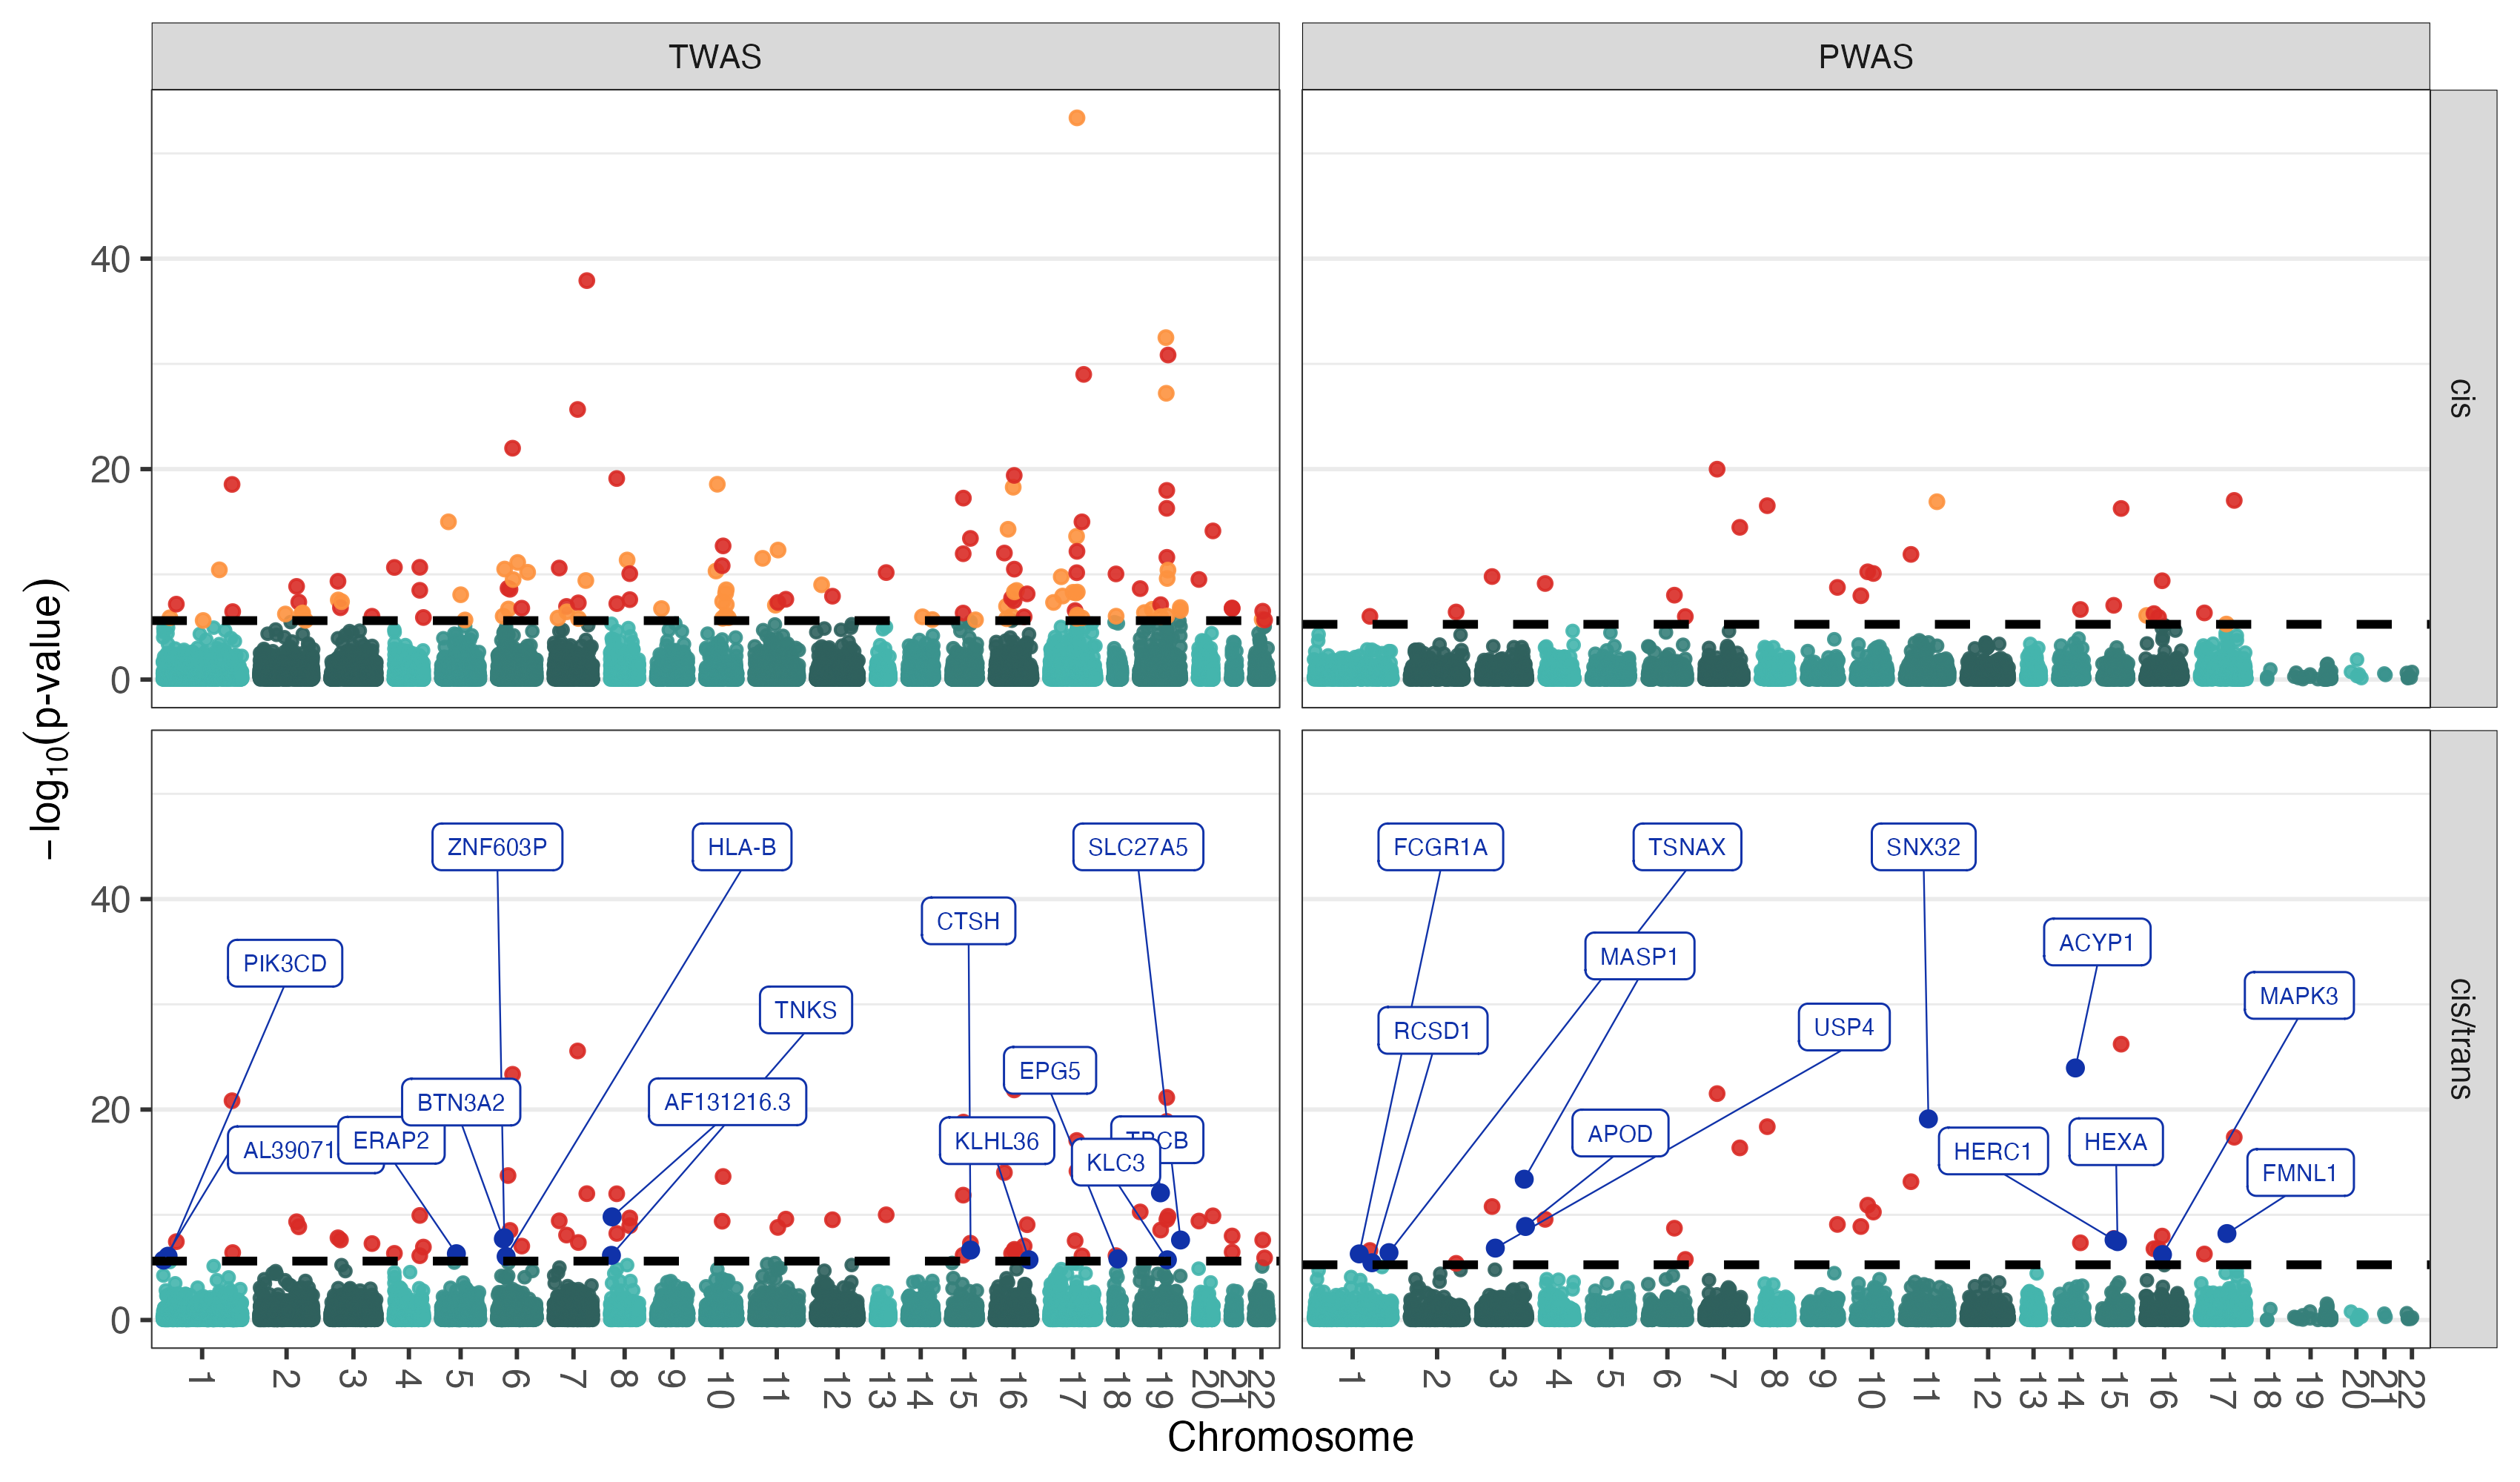
\includegraphics[width=\textwidth]{../figs/manplots_report.png}
  \label{fig:manplot}
  {\footnotesize
  Significant genes identified by only the \textit{cis}/\textit{trans} xWASs are labeled and shown in blue. Significant genes identified by both the \textit{cis}- and \textit{cis}/\textit{trans} models for a given xWAS (TWAS or PWAS) are shown in red. All other significant genes are shown in orange. Non-significant genes are shown in green.}
\end{figure}



Figure~\ref{fig:venn} shows a venn diagram of overlapping risk genes identified by these four xWAS studies: 4 genes (\textit{ACE}, \textit{EGFR}, \textit{EPHX2}, \textit{LACTB}) were identified by all four studies and another 5 (\textit{CTSH}, \textit{EARS2}, \textit{FCER1G}, \textit{LARS2}, \textit{SNX32}) were identified by at least three of the four xWASs. With the exception of known AD TWAS risk gene \textit{LARS2}~\cite{qianRegulatingLars2Mitochondria2024}, these genes have been previously identified as GWAS risk genes of AD. These risk, as well as a brief description of any known functions, is in Table~\ref{tab:multixwasriskgenes}. Other previously identified GWAS and TWAS risk genes of AD that have been replicated here include \textit{CR1}, \textit{HLA-DRA}, and \textit{MAPT-AS1}~\cite{parrishSRTWASLeveragingMultiple2024b}. 

\begin{table}[H]\centering
	\caption{Risk Genes Identified by 3 or more xWAS}
  \begin{tabular}{lll}
    \toprule
     CHR &   Gene &  Function/Disease Association \\ \midrule
      1 & \textit{FCER1G}* & immunoreceptor \\
      % \only<beamer>{\only<1>{3 & \textit{LARS2} & catalyzes attachment of amino acid Leu to tRNA \\}}
      % \onslide<2->{\textbf{3} & \textbfit{LARS2} & \textbf{catalyzes attachment of amino acid Leu to tRNA} \\}
      3 & \textit{LARS2}** & catalyzes attachment of amino acid Leu to tRNA \\
      7 & \textit{EGFR}* & epidermal growth factor receptor \\
      8 & \textit{EPHX2}* & lipid mediator; mutations associated with familial hypercholesterolemia \\
      11 & \textit{SNX32}* & may be involved intercellular trafficking \\
      15 & \textit{LACTB}* & regulator of mitochondrial lipid metabolism \\
      15 &  \textit{CTSH}* & degradation of proteins in lysosomes \\
      16 & \textit{EARS2}* & catalyzes attachment of amino acids Glu and Gln to mitochondrial tRNAs \\
      17 & \textit{ACE}* & angiotensin-converting enzyme \\
    \bottomrule
    \multicolumn{3}{l}{\footnotesize $\ast$ previously-identified GWAS risk genes} \\
    \multicolumn{3}{l}{\footnotesize $\ast\ast$ TWAS risk gene of AD, potential drug target}\cite{qianRegulatingLars2Mitochondria2024}
  \end{tabular}
  \label{tab:multixwasriskgenes}
\end{table}

\begin{figure}[H]\centering
\caption{Venn Diagrams of Overlapping xWAS Results}
  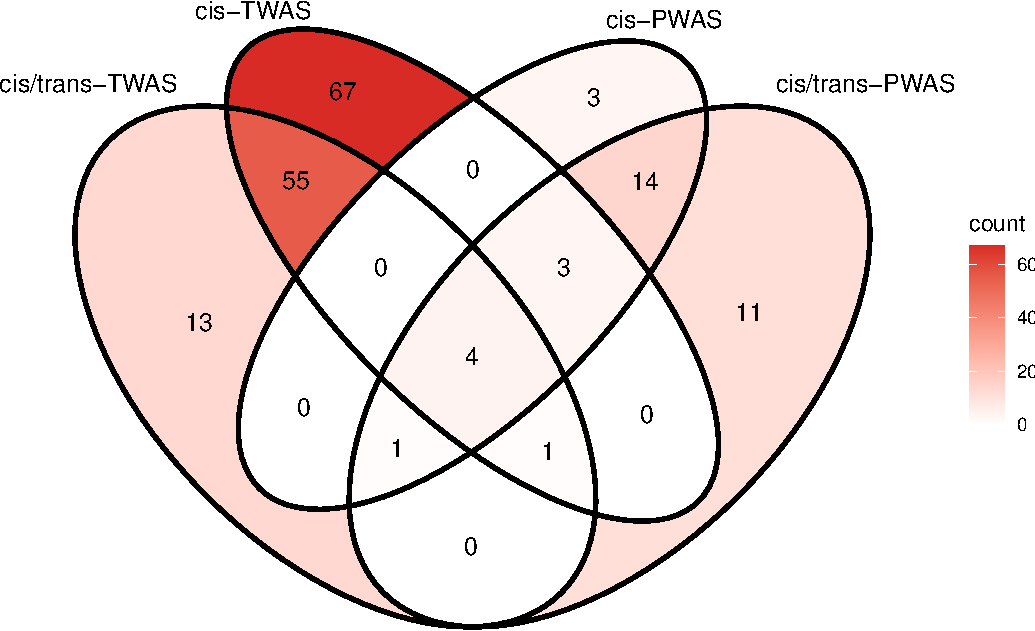
\includegraphics[width=0.8\textwidth]{../figs/venn_report-crop.pdf}
  \label{fig:venn}
\end{figure}

PathDIP~\cite{pastrelloPathDIP5Improving2024} was used to perform enrichment analyses on the risk genes obtained from the four xWAS. Significantly enriched pathways for each are shown in Figure~\ref{fig:paths_plot} while Figure~\ref{fig:paths_venn} shows the number of significant enriched pathways shared across the xWASs; there were 5 pathways significantly enriched for all xWASs (Table~\ref{tab:allenriched}).


% \begin{table}[H]\centering
% 	\caption{xWAS Association Test Results Summary}
%   \begin{tabular}{lrrrrr}
%     \toprule
%      &  Total Genes &   Significant &  Nonsignificant & NA &  \textit{trans}-only \\ \midrule
%     cis-TWAS &  16408 &   130 &   15973 &   305 &   0 \\
%     cis/trans-TWAS &  16676 &   74 &  16047 &   555 &   298 \\[0.25em]
%     cis-PWAS &  8829 &  25 &  7553 &  1251 &  0 \\
%     cis/trans-PWAS &  8922 &  34 &  7595 &  1293 &  84 \\
%     \bottomrule
%   \end{tabular}
%   \label{tab:summary}
% \end{table}



\section{Summary}

Traditional xWAS studies neglect \textit{trans}-QTLs which can explain a significant amount of variation of expression quantitative traits and explain underlying biological mechanisms, but the associated computational burden renders routine methods non-feasible. The BGW-xWAS tool was developed to reduce computational burden of incorporating \textit{trans}-QTLs into the standard two-stage xWAS model. Application studies of AD xWAS show risk genes significantly enriched for AD-related pathways, including Alzheimer disease-amyloid secretase path. 

BGW-TWAS does have some limitations: it assumes a two-stage model for xWASs and computational costs are still substantial to train models for genome-wide genes per tissue type, per -omic data type: it takes approximately 30min of computation time per gene (in parallel with 4 CPU cores). BGW-PWAS considers only protein abundance and does not consider the effect of genetic variants on protein function~\cite{brandesPWASProteomewideAssociation2020}.


% % REFERENCE SECTION
% \newpage
\pagebreak

\renewcommand\bibsection{\section{\refname}}
% \bibliographystyle{abbrvnat-maxbibnames4}
\bibliographystyle{abbrvnat-maxbibnames4_sortnumeric}
% \bibliographystyle{unsrtnat}
% \bibliographystyle{plain}
% \bibliographystyle{natbib}
\bibliography{biblio} %Example
% \printbibliography[heading=none] 
\newpage
%%%%%
\pagebreak
% \begin{center} \Large \textbf{Appendix} \end{center}

%% Appendix
\begin{appendices}


\section{Figures}




% \begin{figure}[H]\centering
% 	\caption{Manhattan Plots of xWAS Results}
%   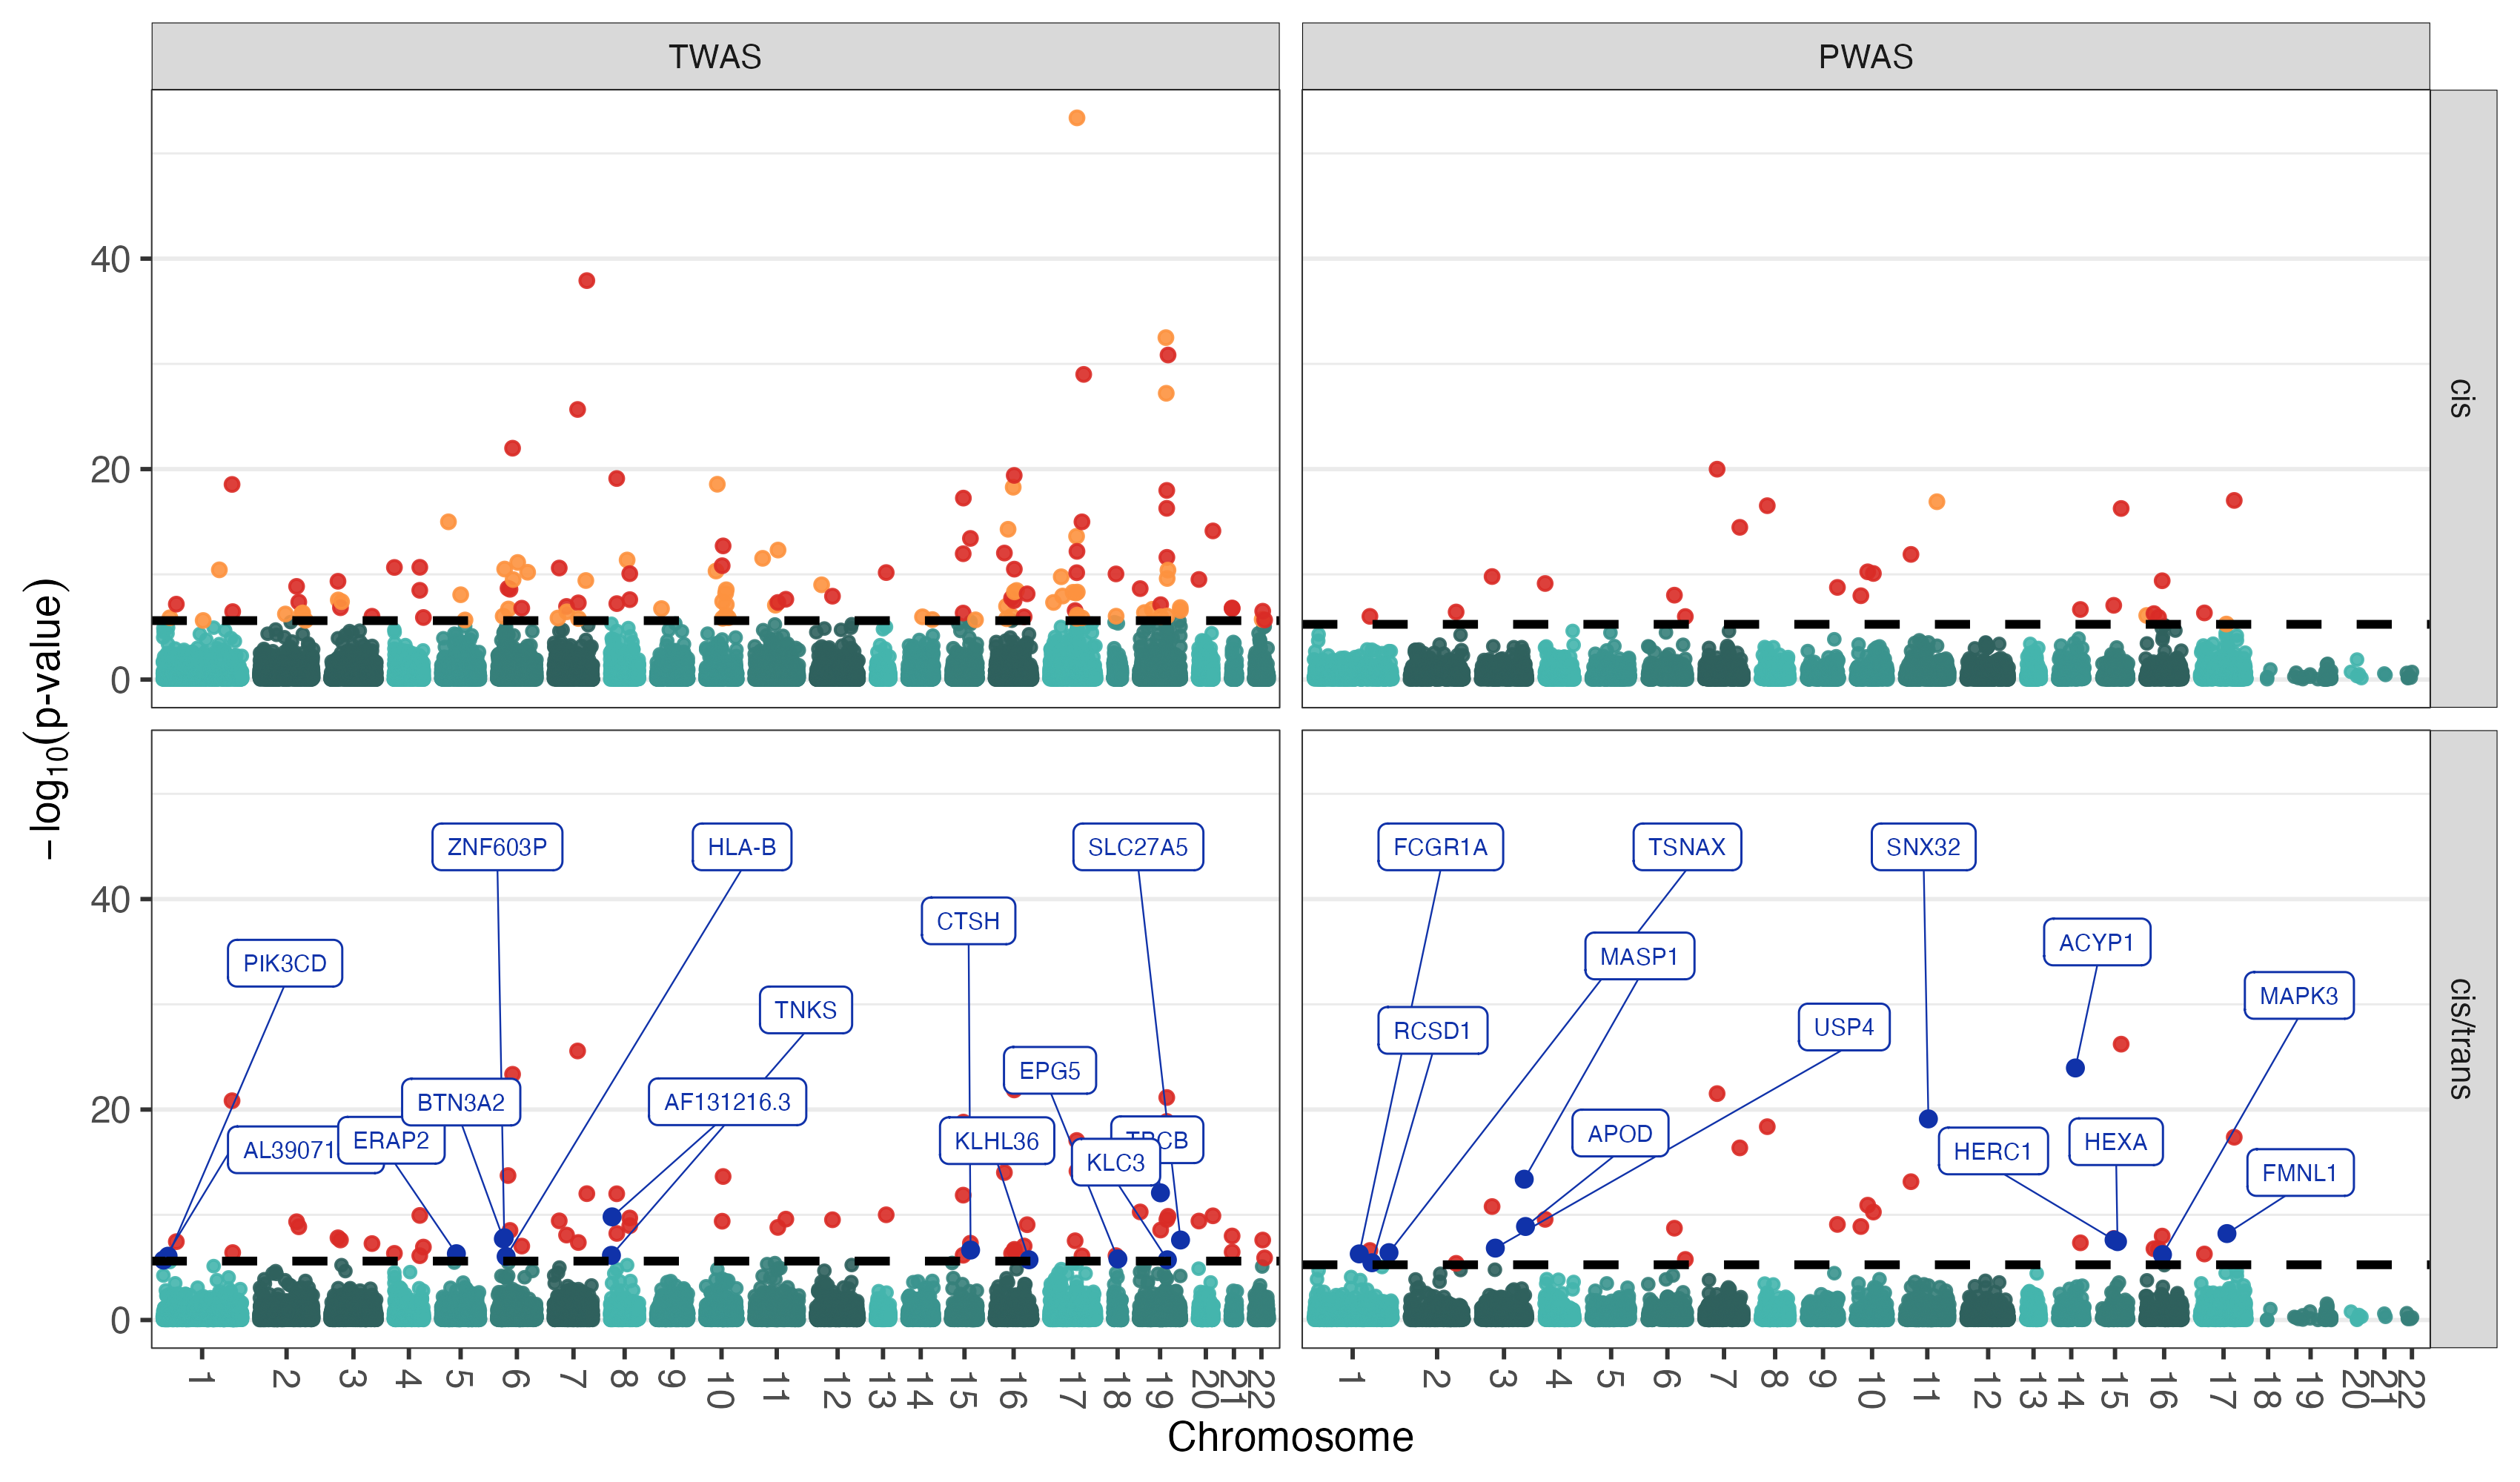
\includegraphics[width=\textwidth]{../figs/manplots_report.png}
%   \label{fig:manplot}
%   {\footnotesize
%   Significant genes identified by only the \textit{cis}/\textit{trans} xWASs are labeled and shown in blue. Significant genes identified by both the \textit{cis}- and \textit{cis}/\textit{trans} models for a given xWAS (TWAS or PWAS) are shown in red. All other significant genes are shown in orange. Non-significant genes are shown in green.}
% \end{figure}



% \begin{figure}[H]\centering
% \caption{Venn Diagrams of Overlapping xWAS Results}
%   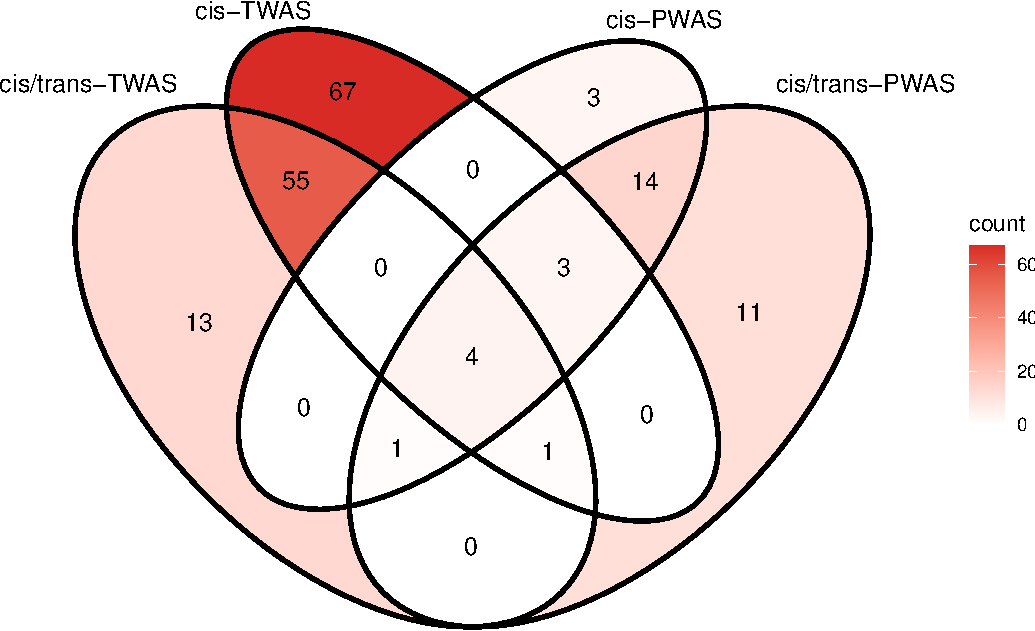
\includegraphics[width=0.8\textwidth]{../figs/venn_report-crop.pdf}
%   \label{fig:venn}
% \end{figure}


\begin{figure}[H]\centering
	\caption{Significant Enriched Paths by pathDIP}
  \includegraphics[width=\textwidth]{../figs/paths_plot.png}
  \label{fig:paths_plot}
\end{figure}


\begin{figure}[H]\centering
	\caption{Venn Diagram of Number of Overlapping Paths for each xWAS}
  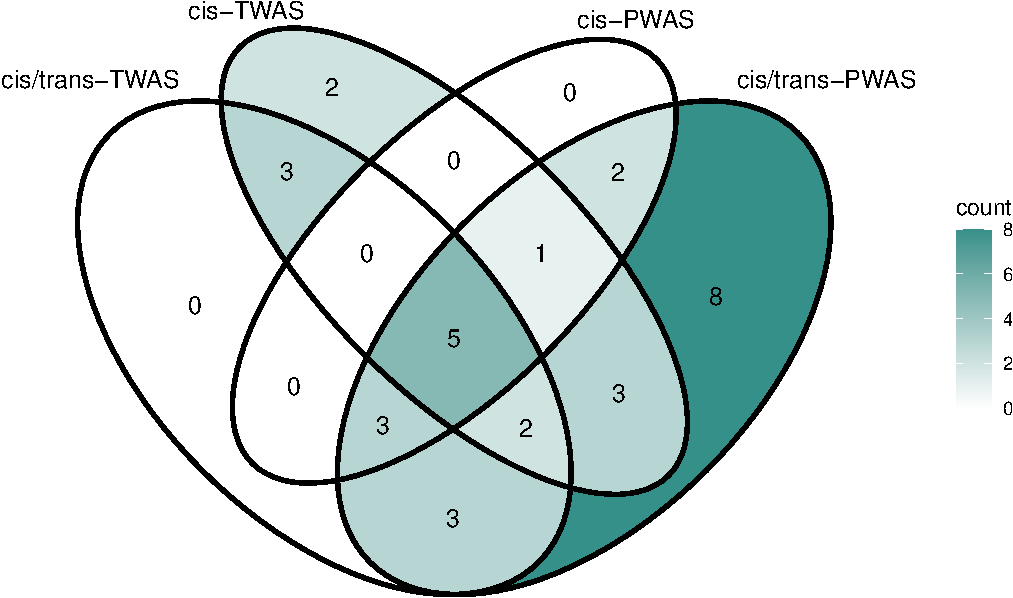
\includegraphics[width=0.8\textwidth]{../figs/paths_venn_report-crop.pdf}
  \label{fig:paths_venn}
\end{figure}




\section{Tables}
\input{report_tables.tex}


\end{appendices}
\end{document}
